\documentclass[12pt, a4paper, oneside, final]{article}
\usepackage[margin = 1in, bottom = 1in]{geometry}

\usepackage[T2A]{fontenc}
\usepackage[utf8]{inputenc}
\usepackage[english, russian]{babel}
\usepackage{xcolor, ulem, soulutf8, soul, fancyhdr, amsmath, amssymb, amsthm, svg, wrapfig, csvsimple, float, caption, subcaption}
\usepackage[shortlabels]{enumitem}
\usepackage{titlesec, hyperref, multicol, listings}
\usepackage[most]{tcolorbox}
\usepackage[makeroom]{cancel}
\usepackage[most]{tcolorbox}
\usepackage{tocloft, longtable, skak, stmaryrd, color}
\usepackage[framemethod = tikz]{mdframed}
\usepackage{minted}

\definecolor{codegreen}{rgb}{0,0.6,0}
\definecolor{codegray}{rgb}{0.5,0.5,0.5}
\definecolor{codepurple}{rgb}{0.58,0,0.82}
\definecolor{backcolour}{rgb}{0.95,0.95,0.92}
\definecolor{blueish}{rgb}{0.96,0.96,1.0}
\definecolor{grayblueish}{rgb}{0.97,0.97,0.98}
\definecolor{transblue}{rgb}{0.9,0.9,0.97}
\definecolor{transred}{rgb}{0.97,0.9,0.9}
\definecolor{light-gray}{gray}{0.95}

\renewcommand{\figurename}{}
\addto\captionsrussian{\renewcommand{\figurename}{}}
\captionsetup[table]{labelformat = empty}

\hypersetup{
	colorlinks,
	citecolor = pink,
	filecolor = pink,
	linkcolor = pink,
	urlcolor = pink
}

\newtcblisting{mylisting}{
	listing only,
	breakable,
	colback = backcolour,
	enhanced jigsaw,
	sharp corners,
	boxrule = 0pt,
	frame hidden,
	listing options = {
		mathescape,
		commentstyle = \color{codegreen},
		keywordstyle = \color{magenta},
		numberstyle = \tiny\color{codegray},
		stringstyle = \color{codepurple},
		basicstyle = \ttfamily\footnotesize,
		breakatwhitespace = false,
		breaklines = true,
		captionpos = b,
		keepspaces = true,
		numbers = left,
		numbersep = 5pt,
		showspaces = false,
		showstringspaces = false,
		showtabs = false,
		tabsize = 4,
		inputencoding = utf8,
		language = python
	}
}

\binoppenalty = 10000
\relpenalty = 10000
\sloppy

\renewcommand*{\theenumi}{\thesection.\arabic{enumi}}
\renewcommand*{\theenumii}{\alph{enumii}}
\renewcommand*{\labelitemi}{\ensuremath{\triangleright}}

\everymath{\displaystyle}

\begin{document}
	\thispagestyle{empty}
	\vspace*{0.5em}
	\begin{center}
		{Национальный исследовательский университет ИТМО\\Факультет информационных технологий и программирования\\Прикладная математика и информатика}\\[5.0em]
		{\Huge \bfseries Методы оптимизации}\\[0.5em]
		{\large Отчет по лабораторной работе №4}\\[0.5em]
		\textcolor{gray}{\textlangle Собрано \today\textrangle}
	\end{center}
	\begingroup
	\def\hd{\begin{tabular}{ll}
			\textbf{Работу выполнили:} \\ Бактурин Савелий Филиппович M32331 \\ Вереня Андрей Тарасович M32331 \\ Сотников Максим Владимирович M32331 \vspace*{1em} \\
			\textbf{Преподаватель:} \\ Казанков Владислав Константинович
		\end{tabular}
	}
	\vspace*{30em}
	\newlength{\hdwidth}
	\settowidth{\hdwidth}{\hd}
	\hfill\begin{minipage}{\hdwidth}\hd\end{minipage}
	\endgroup
	\newpage
	\section*{Стохастический градиентный спуск vs. \texttt{torch.optim}}
	Настало время сравнить самописные реализации обычного и других модифицированных версий стохастического градиентного спуска с написанным серьезным дядьками из PyTorch.
	В качестве экспериментирования мы возьмем старую добрую функцию Розенброка, которая на плоскости $\mathbb{R}^2$ определяется следующим образом:
	\[
		f(x, ~ w_0, ~ w_1) = (1 - x \cdot x_0)^2 + 100 \cdot (x \cdot w_1 - x^2)^2,
	\] где $w_0$ и $w_1$~-- некие конечные константы.
	Теперь установим некие параметры для будущих тестов, а именно для генерации набора данных (\textit{dataset}):
	\begin{align*}
		\mathit{\mathtt{density}} &= 8000~\text{(плотность генерируемых точек)}, \\
		\mathit{\mathtt{dots\_count}} &= 1000~\text{(количество генерируемых точек)}, \\
		\mathit{\mathtt{radius}} &= 0.001~\text{(радиус от функции генерации точек)}, \\
		\mathit{\mathtt{dist}} &= 0.01~\text{(расстояние относительно прямой генерации точек)}
	\end{align*}
	Также зададим постоянными параметрами двух конечных констант для функции Розенброка:
	\[
		w_0 = 2 \qquad w_1 = 3
	\]
	Далее количество тестов на усреднение результатов~-- данный параметр говорит, сколько необходимо сделать независимых генераций и запусков алгоритмов с начальной точки нужно сделать, затем усреднить:
	\[
		\mathit{\mathtt{test\_count}} = 100
	\]
	Наконец, зададим начальную точку.
	Поскольку наша задача состоит в исследовании работы алгоритмов в условиях генерируемых новых точек, умоляя тех или иных дополнительных эффектов от \texttt{numpy}-генерации, то мы будем брать в качестве начала одну и ту же точку:
	\[
		\mathit{\mathtt{initial\_w}} = \langle -1.0, ~ 0.1\rangle
	\]
	Перед тем как мы обратимся непосредственно к самим результатам исследований скажем несколько слов по поводу реализуемых и используемых функций.
	По сути, \texttt{torch.optim} это такой конструктор, который необходимо собрать, чтобы получить подходящую под задачу модель.
	В частности реализация использует в качестве подсчета на dataset функцию \texttt{helper.train\_torch\_optim}:
	\begin{align*}
		\mathtt{function}~train\_torch\_optim(&f\ :\ \mathbb{R}^{k + 1} \to \mathbb{R}, \\
		& X_{\text{train}} \subset \mathbb{R}, \\
		& Y_{\text{train}} \subset \mathbb{R}, \\
		& \varepsilon_{\text{minimum}} \in \mathbb{R}, \\
		& \langle x_0, ~ y_0 \rangle \in \mathbb{R}^2, \\
		& g_{\text{loss}}\ :\ \mathbb{R}^{k + 1} \to \mathbb{R}, \\
		& \mathtt{optimizer\_method}\ :\ \text{/*}implementation~defined\text{*/}, \\
		& \mathtt{num\_epochs}~(= 10000) \in \mathbb{N}, \\
		& \mathtt{learning\_rate}~(= 0.01) \in \mathbb{N}, \\
		& \mathtt{momentum}~(= \varnothing) \in \mathbb{R}, \\
		& \mathtt{nesterov}~(= \textit{False}) \in \mathbb{V}, \\
		& \mathtt{apply\_min}~(= \textit{True}) \in \mathbb{V})
	\end{align*}
	По сути, она выстраивает модель оптимизатора, определенный в библиотеке PyTorch, от $\mathtt{optimizer\_method}$, который подается как дождь - с небес, и далее по количестве, ограниченных по умолчанию в 10000 шагов, начинает обновлять параметры модели (от исходной точки) от композиции обнуления градиенты, вычисления функции потерь, проверки на сходимость и, соответственно, шага.
	Наконец, определим еще одну, усредняющую функцию, для вывода результатов~-- \texttt{get\_average\_loss\_history}~-- она вычисляет среднее значение функции потерь \texttt{helper.mse\_loss}, определяемая как
	\begin{mylisting}
function $mse\_loss(X_{\text{dataset}}, ~ Y_{\text{dataset}}, ~ w, ~ f)$:
	$y' \gets \mathtt{f}(X_{\text{dataset}}, ~ w)$;
	return $\text{torch}.\mathtt{mean}((Y_{\text{dataset}} - y')^2)$;
	\end{mylisting}
	То есть, такая функция, которая вычисляет среднеквадратичную ошибку между предсказанными и реальными значениями на основе модели.
	\subsection*{SGD vs. \mintinline{python}|torch.optim.SGD|}
	Перейдем к исследованиям.
	Первым на подходе мы посмотрим на стандартный стохастический градиентный спуск (с размером батча, равный единице).
	Запустим наших зверей и посмотрим на вывод в виде графика, по оси Y которой мы выставим значения функции потерь, по оси X~- количество шагов до остановки алгоритма.
	\begin{figure}[H]
		\centering
		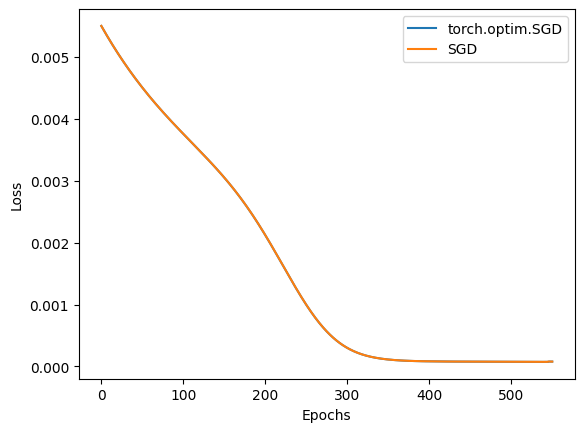
\includegraphics[scale = 1]{Image/T1_SGD_vs_torch_optim_SGD.png}
		\caption*{Implemented SGD vs. PyTorch's}
	\end{figure}
	Графики почти полностью совпали.
	Полученные результаты соответствующие:
	\begin{table}[H]
		\centering
		\begin{tabular}{l|l|l}
			Испытуемый & Значение функции потерь & Среднее число шагов до схождения \\ \hline
			Настоящие данные & $0.00007481586253817499$ & - \\
			\mintinline{python}|torch.optim.SGD| & $0.00007753667274059714$ & $551$ \\
			Собственная реализация & $0.00007756952443600056$ & $551$
		\end{tabular}
	\end{table}
	Как мы видим, значения, особенно количество шагов до схождения алгоритма, почти полностью совпадают.
	Есть теория, что стохастический градиентный спуск был сделан правильно и, как сказал один из коллег по лабораторной работе, <<по другому он не может быть сделан>>.
	По более формальной теории, поскольку dataset используется один и тот же, то есть вероятность, что точки были так удачно распределены даже спустя $100$ тестов, что любая выбранная из батч размера нивелирует среднее значение.
	\subsection*{AdaGrad vs. \mintinline{python}|torch.optim.AdaGrad|}
	С AdaGrad'ом ситуации поинтереснее.
	Запустим наших зверей и посмотрим на вывод в виде графика, по оси Y которой мы выставим значения функции потерь, по оси X~- количество шагов до остановки алгоритма.
	\begin{figure}[H]
		\centering
		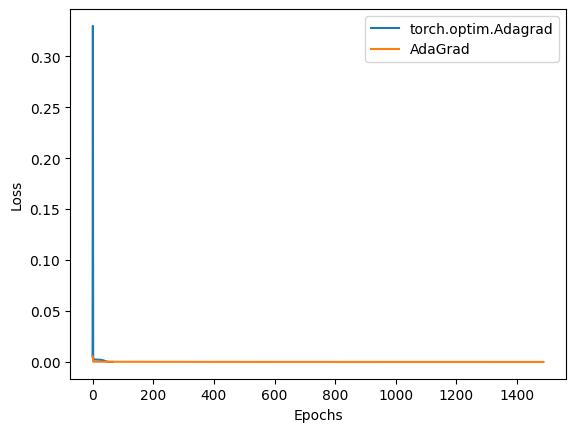
\includegraphics[scale = 1]{Image/T1_ADAGRAD_vs_torch_optim_AdaGrad.png}
		\caption*{Implemented AdaGrad vs. PyTorch's}
	\end{figure}
	Также, для наглядности, немного приблизимся к почти незаметной горке, ограничивая по оси Y.
	\begin{figure}[H]
		\centering
		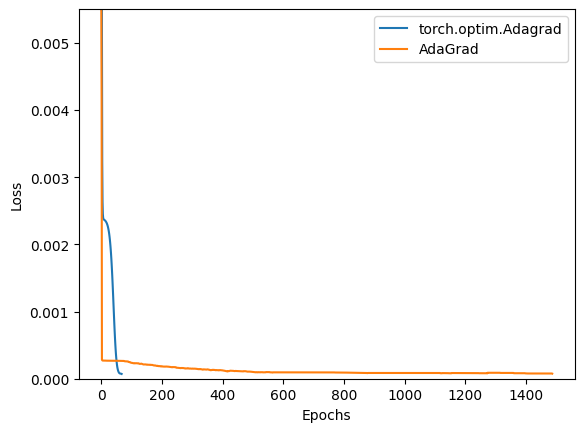
\includegraphics[scale = 1]{Image/T1_ADAGRAD_vs_torch_optim_AdaGrad_ZOOM.png}
		\caption*{Implemented AdaGrad vs. PyTorch's (zoom)}
	\end{figure}
	Полученные результаты соответствующие:
	\begin{table}[H]
		\centering
		\begin{tabular}{l|l|l}
			Испытуемый & Значение функции потерь & Среднее число шагов до схождения \\ \hline
			Настоящие данные & $0.00007481586253817499$ & - \\
			\mintinline{python}|torch.optim.AdaGrad| & $0.00007116629643237779$ & $68$ \\
			Собственная реализация & $0.00007581577268337732$ & $1488$
		\end{tabular}
	\end{table}
	Ситуация обратная самому первому исследованию: собственная реализация сильно проигрывает библиотечной.
	Это происходит из-за неправильно установленного изначально $\texttt{learning\_rate}$, отчего своя реализация уходит в небытие.
	Также, существует мнение, что библиотечная функция рассчитана на <<неудобные>> начальные данная (что-то вроде защиты от дураков).
	А поскольку в нашем случае такого не предполагалось (вернее, обработки столь щепетильной ситуации), то и в реализации такого и нету.
	\subsection*{Momentum vs. \mintinline{python}|torch.optim.SGD| (with \mintinline{python}|momentum = True|)}
	От более сложной модели мы перейдем, внезапно, к самой простой модификации к стохастическому градиентному спуску, основанный на физических моделях момента Momentum.
	Запустим наших зверей и посмотрим на вывод в виде графика, по оси Y которой мы выставим значения функции потерь, по оси X~- количество шагов до остановки алгоритма.
	\begin{figure}[H]
		\centering
		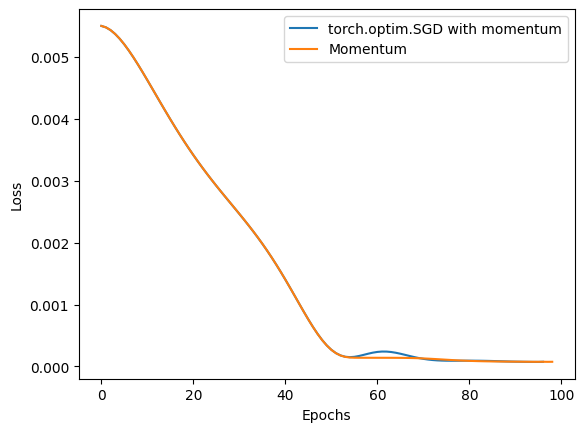
\includegraphics[scale = 1]{Image/T1_MOMENTUM_vs_torch_optim_SGD_MOMENTUM.png}
		\caption*{Implemented Momentum vs. PyTorch's}
	\end{figure}
	Полученные результаты соответствующие:
	\begin{table}[H]
		\centering
		\begin{tabular}{l|l|l}
			Испытуемый & Значение функции потерь & Среднее число шагов до схождения \\ \hline
			Настоящие данные & $0.00007481586253817499$ & - \\
			\mintinline{python}|momentum = True| & $0.00007458029055847868$ & $97$ \\
			Собственная реализация & $0.00007460658043034181$ & $99$
		\end{tabular}
	\end{table}
	Замечаем, что результаты, в особенности среднее значение функции потерь, почти не изменилось.
	В отличие от количества шагов, который совершенно мало увеличилось, что, опять же, как и в предыдущем случае, может быть связано с кривым поданным \texttt{learning\_rate}.
	И всё же, почему полученные значения почти совпадают?
	Ситуация аналогична с ситуацией при исследовании обычного стохастического спуска: простота написания функции уменьшает количество ошибок и неточностей далее.
	\subsection*{Nesterov vs. \mintinline{python}|torch.optim.SGD| (with \mintinline{python}|momentum = True|, \mintinline{python}|nesterov = True|)}
	В реализации библиотеки PyTorch функция SGD, для работы того самого Nesterov требует два флага: \mintinline{python}|momentum| и \mintinline{python}|nesterov|~-- это объясняется тем, модификация Nesterov берет за основу и использует идею Momentum.
	Запустим наших зверей и посмотрим на вывод в виде графика, по оси Y которой мы выставим значения функции потерь, по оси X~- количество шагов до остановки алгоритма.
	\begin{figure}[H]
		\centering
		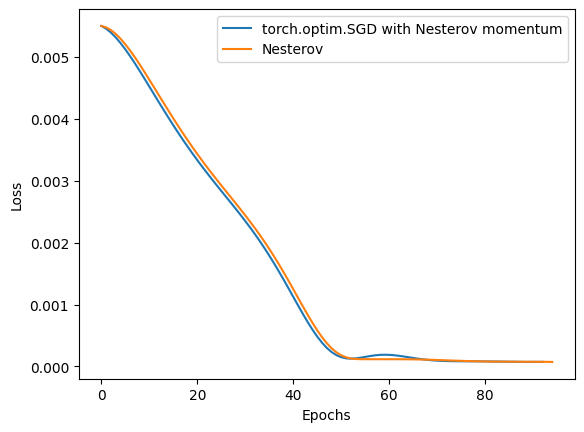
\includegraphics[scale = 1]{Image/T1_NESTEROV_vs_torch_optim_SGD_NESTEROV.png}
		\caption*{Implemented Nesterov vs. PyTorch's}
	\end{figure}
	Полученные результаты соответствующие:
	\begin{table}[H]
		\centering
		\begin{tabular}{l|l|l}
			Испытуемый & Значение функции потерь & Среднее число шагов до схождения \\ \hline
			Настоящие данные & $0.00007458029055847868$ & - \\
			\mintinline{python}|nesterov = True| и ... & $0.00007412807086024441$ & $93$ \\
			Собственная реализация & $0.00007271430540397701$ & $95$
		\end{tabular}
	\end{table}
	Ситуация аналогична с предыдущим исследованием: наши средние значения функции потерь также почти одинаковы, отличаемые лишь в шестой цифре, и по среднему число шагов до схождения, отличаемые лишь на некоторую константу.
	Полученные эквивалентные результаты обусловлены простотой реализации данной модификации к стохастическому градиентному спуску.
	\subsection*{RMSProp vs. \mintinline{python}|torch.optim.RMSProp|}
	А вот мы и добрались до того самого момента, когда самописная реализация выходит победителем в межвидовой борьбе.
	Рассмотрим одного из двух гигантов модификаций~-- RMSProp.
	Запустим наших зверей и посмотрим на вывод в виде графика, по оси Y которой мы выставим значения функции потерь, по оси X~- количество шагов до остановки алгоритма.
	\begin{figure}[H]
		\centering
		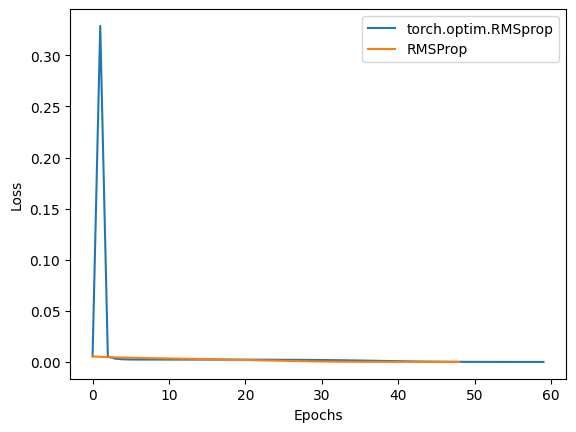
\includegraphics[scale = 1]{Image/T1_RMSPROP_vs_torch_optim_RMSPROP.png}
		\caption*{Implemented RMSProp vs. PyTorch's}
	\end{figure}
	Также, для наглядности, немного приблизимся к почти незаметной горке, ограничивая по оси Y.
	\begin{figure}[H]
		\centering
		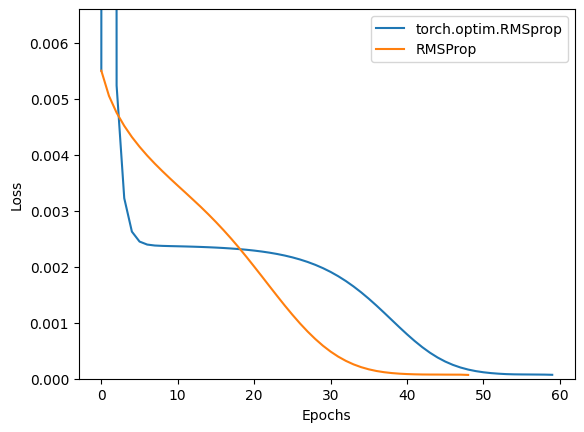
\includegraphics[scale = 1]{Image/T1_RMSPROP_vs_torch_optim_RMSPROP_ZOOM.png}
		\caption*{Implemented RMSProp vs. PyTorch's (zoom)}
	\end{figure}
	Полученные результаты соответствующие:
	\begin{table}[H]
		\centering
		\begin{tabular}{l|l|l}
			Испытуемый & Значение функции потерь & Среднее число шагов до схождения \\ \hline
			Настоящие данные & $0.00007481586253817499$ & - \\
			\mintinline{python}|torch.optim.RMSProp| & $0.00007001601600272134$ & $60$ \\
			Собственная реализация & $0.00006762658137925631$ & $49$
		\end{tabular}
	\end{table}
	Неожиданно, теперь в исследовании мы получаем обратную картину об общем строении мира.
	Дело в том, что мы все это время имели в том или ином смысле функции, которые направлены на решение более общих задач, даже для случаев, когда в функцию минимизации намеренно дают <<плохой>> вариант \texttt{learning\_rate}, она за конечное число шагов выровняет в нормальный размер шага.
	Однако, посматривая на реализацию \mintinline{python}|torch.optim.RMSProp| \url{https://pytorch.org/docs/stable/generated/torch.optim.RMSprop.html}, мы понимаем, что есть некоторые параметры, которые оказались никоим образом не тронутые в исследовании и возможно они бы уменьшили число шагов до или даже меньше собственной реализации.
	С другой стороны, поскольку предоставленные значения все же являются усредненными, мы можем предположить, что та $\delta$-разница между средним числом шагов своей реализации и библиотечной, является константной и никуда не меняется (следовательно, если бы мы немного изменили начальный шаг, мы бы получили совершенно иные результаты).
	\subsection*{Adam vs. \mintinline{python}|torch.optim.Adam|}
	Еще один гигант и еще одна жертва падения (на самом деле, не совсем) перед своей реализацией библиотечной версии.
	Запустим наших зверей и посмотрим на вывод в виде графика, по оси Y которой мы выставим значения функции потерь, по оси X~- количество шагов до остановки алгоритма.
	\begin{figure}[H]
		\centering
		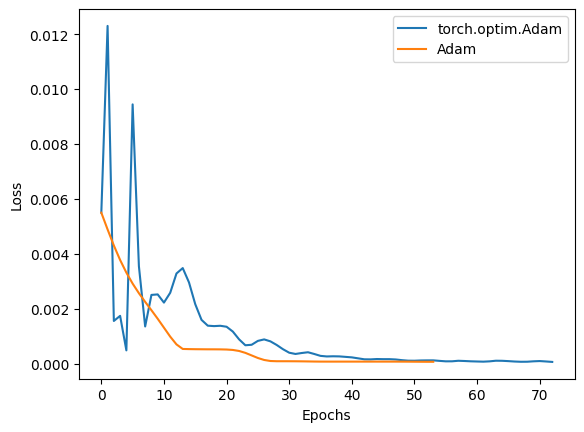
\includegraphics[scale = 1]{Image/T1_ADAM_vs_torch_optim_ADAM.png}
		\caption*{Implemented Adam vs. PyTorch's}
	\end{figure}
	Полученные результаты соответствующие:
	\begin{table}[H]
		\centering
		\begin{tabular}{l|l|l}
			Испытуемый & Значение функции потерь & Среднее число шагов до схождения \\ \hline
			Настоящие данные & $0.00007481586253817499$ & - \\
			\mintinline{python}|torch.optim.Adam| & $0.00006828866230090804$ & $73$ \\
			Собственная реализация & $0.00007292588434103817$ & $54$
		\end{tabular}
	\end{table}
	Казалось бы, свой Adam побеждает в числе шагов до вхождения, но тут мы внезапно осознаем, что не все так просто, как кажется.
	Дело в том, что библиотечный Adam, внезапно, оказывается куда точнее, нежели чем тем же настоящие данные и своя реализация.
	Это связано опять же с нашим вездесущим другом по имени \texttt{learning\_rate}, если в собственная функция, вероятнее всего, по задумке изученного алгоритма, считает правильно точно, то вот новый, который по документации~-- \url{https://pytorch.org/docs/stable/generated/torch.optim.Adam.html}~-- включает в себя дополнительный, еще один, последний, \mintinline{python}|if| возвращает, очевидно, еще более точный минимум.
	Объяснение, почему количество шагов в реализации с нуля оказывается меньше, чем в библиотечной функции, аналогично предыдущем суждениям.
	\subsection*{Дополнительные исследования}
	Дальнейшие исследования не буду включать в себя многословные попытки объяснит, что к чему, а лишь будут иметь информативные представления о том, какие функции используются и какие результаты по итогам исследования вышли.
	Данный блок скорее нужен только для того, чтобы увидеть разницу между методами и их работой на общей поле битвы.
	\subsubsection*{Nesterov vs. SGD vs. \mintinline{python}|torch.optim.SGD| vs. \mintinline{python}|torch.optim.SGD| (\mintinline{python}|momentum|)}
	Рассмотрим вот такую именитую четверку двух самых простых и неинтересных, двух сражающихся за право быть наименьшим по среднему числу шагов до сходимости: SGD и \mintinline{python}|torch.optim.SGD|, Nesterov и \mintinline{python}|torch.optim.SGD| (с \mintinline{python}|momentum = True| и \mintinline{python}|nesterov = True|).
	Запустим наших зверей и посмотрим на вывод в виде графика, по оси Y которой мы выставим значения функции потерь, по оси X~- количество шагов до остановки алгоритма.
	\begin{figure}[H]
		\centering
		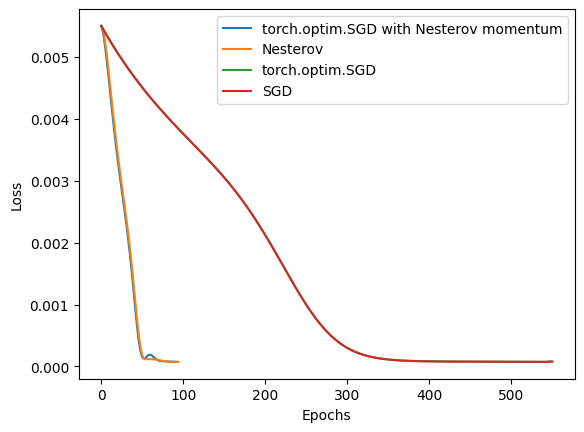
\includegraphics[scale = 1]{Image/T1_SGD_vs_PYTORCH-SGD_vs_NESTEROV_vs_PYTORCH-NESTEROV.png}
		\caption*{Implemented SGD and Nesterov vs. PyTorch's}
	\end{figure}
	Полученные результаты соответствующие:
	\begin{table}[H]
		\centering
		\begin{tabular}{l|l|l}
			Испытуемый & Значение функции потерь & Среднее число шагов до схождения \\ \hline
			Настоящие данные & $0.00007481586253817499$ & - \\
			\mintinline{python}|nesterov = True| и ... & $0.00007292588434103817$ & $93$ \\
			Свой Nesterov & $0.00007271430540397701$ & $95$ \\
			\mintinline{python}|torch.optim.SGD| & $0.00007753667274059714$ & $551$ \\
			Свой SGD & $0.00007756952443600056$ & $551$
		\end{tabular}
	\end{table}
	\subsubsection*{Хаос}
	А теперь выпустим всех зверей наружу кроме трех неудачников, чтобы график не выглядел слишком плохо и ужасно: SGD (свой), \mintinline{python}|torch.optim.SGD| и AdaGrad (свой).
	\begin{figure}[H]
		\centering
		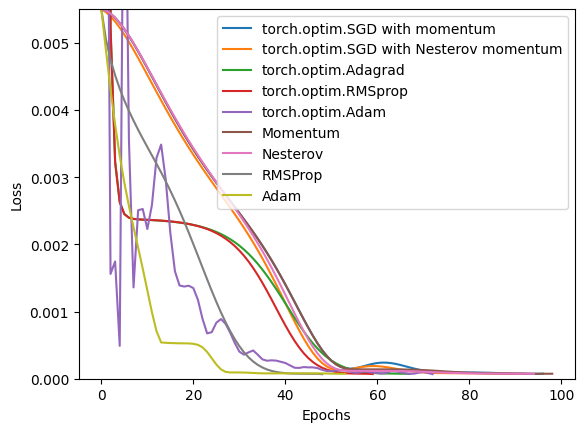
\includegraphics[scale = 1]{Image/T1_CHAOS.png}
		\caption*{Implemented almost everyone vs. PyTorch's}
	\end{figure}
	Полученные результаты соответствующие:
	\begin{table}[H]
		\centering
		\begin{tabular}{l|l|l}
			Испытуемый & Значение функции потерь & Среднее число шагов до схождения \\ \hline
			Настоящие данные & $0.00007481586253817499$ & - \\
			\mintinline{python}|momentum = True| & $0.00007458029055847868$ & $97$ \\
			\mintinline{python}|nesterov = True| и ... & $0.00007412807086024441$ & $93$ \\
			\mintinline{python}|torch.optim.AdaGrad| & $0.00007116629643237779$ & $68$ \\
			\mintinline{python}|torch.optim.RMSProp| & $0.00007001601600272134$ & $60$ \\
			\mintinline{python}|torch.optim.Adam| & $0.00006828866230090804$ & $73$ \\
			Свой Momentum & $0.00007460658043034181$ & $99$ \\
			Свой Nesterov & $0.00007271430540397701$ & $95$ \\
			Свой RMSProp & $0.00006762658137925631$ & $49$ \\
			Свой Adam & $0.00007292588434103817$ & $54$
		\end{tabular}
	\end{table}
	\newpage
	\section*{\mintinline{python}|scipy.optimize.minimize| и \mintinline{python}|scipy.optimize.least_squares|}
	\subsection*{vs. ЛР №3}
	Настала пара проверить эквивалентность работы алгоритмов из великой и ужасной библиотеки SciPy, в котором, в отличии от PyTorch, уже за нас, ленивых разработчиков, сделано в виде удобных функций с бесконечным числом интуитивно понятных параметров.
	Здесь мы хотим рассмотреть и рассмотрим только два метода: BFGS и Powell Dog Leg.
	Почему их?
	С первым все понятно: в идеи работы (и, в каком-то смысле, еще и реализации) он почти эквивалентен своему другу/сопернику, оптимизированному в использовании памяти, L-BFGS.
	А вот со вторым ситуация примерно следующая: дело в том, как мы выяснили с предыдущей рассмотренной лабораторной работы, метод Powell Dog Leg является модифицированной версии Gauss-Newtow и исследования показали, что свой туз в рукаве данный метод не часто использует при работе алгоритма (как правило, при первых $k < n$ шагов, далее~-- Gauss-Newton).
	Именно поэтому мы рассматриваем именно их.
	\subsubsection*{vs. \mintinline{python}|scipy.optimize.minimize|}
	\paragraph{BFGS}
	Начнем с BFGS или, как его еще называют в SciPy, \mintinline{python}|scipy.optimize.minimize(method='BFGS')|.
	Исследуем безымянную функцию $f\ :\ \mathbb{R} \times \mathbb{R} \to \mathbb{R}$, определенную следующим образом:
	\[
		f(x, y) = \sin{\left(\dfrac{1}{2} \cdot x^2 - \dfrac{1}{4} \cdot y^2 + 3\right) \cdot \cos{\left(2 \cdot x + 1 - e^{y}\right)}}
	\]
	В качестве исходного приближения положим точку $\langle x_0, y_0 \rangle = \langle -0.3, -1.4 \rangle$.
	Также, в качестве дополнительных параметров для работы алгоритмов мы положим следующие:
	\begin{align*}
		\mathtt{max\_iter} &= 10~\text{(максимальное количество шагов)} \\
		\varepsilon &= 0.000000001~\text{(условие сходимости)}
	\end{align*}
	Запустим наших зверей на бедную функцию и посмотрим на вывод путей в трехмерном виде:
	\begin{figure}[H]
		\centering
		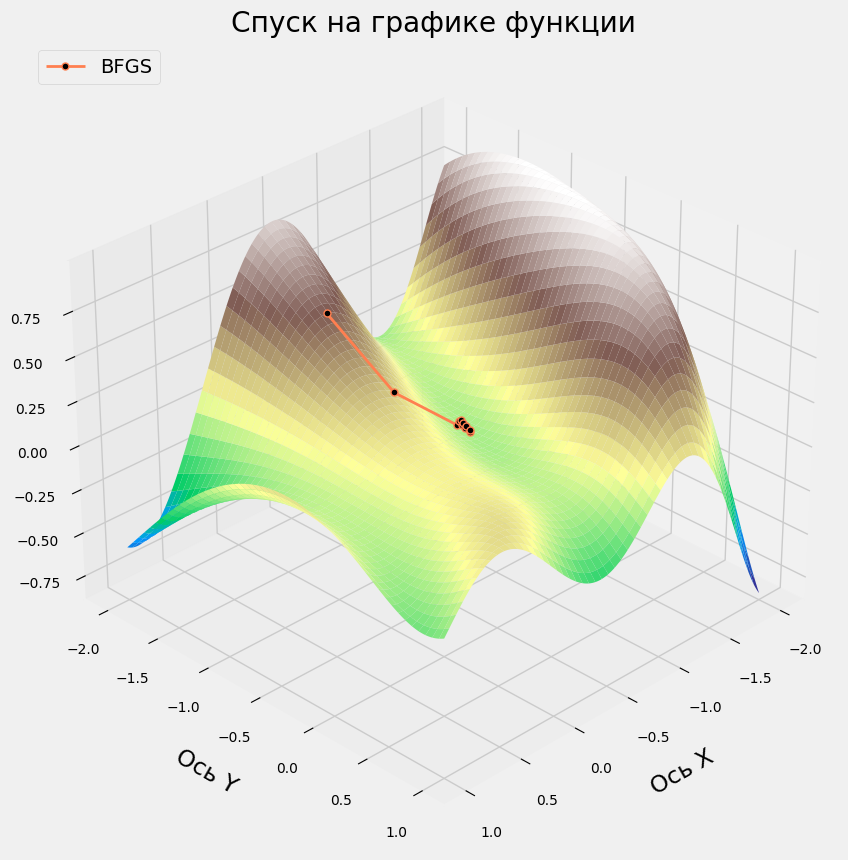
\includegraphics[scale = 0.35]{Image/T2A_F1_BFGS.png}
		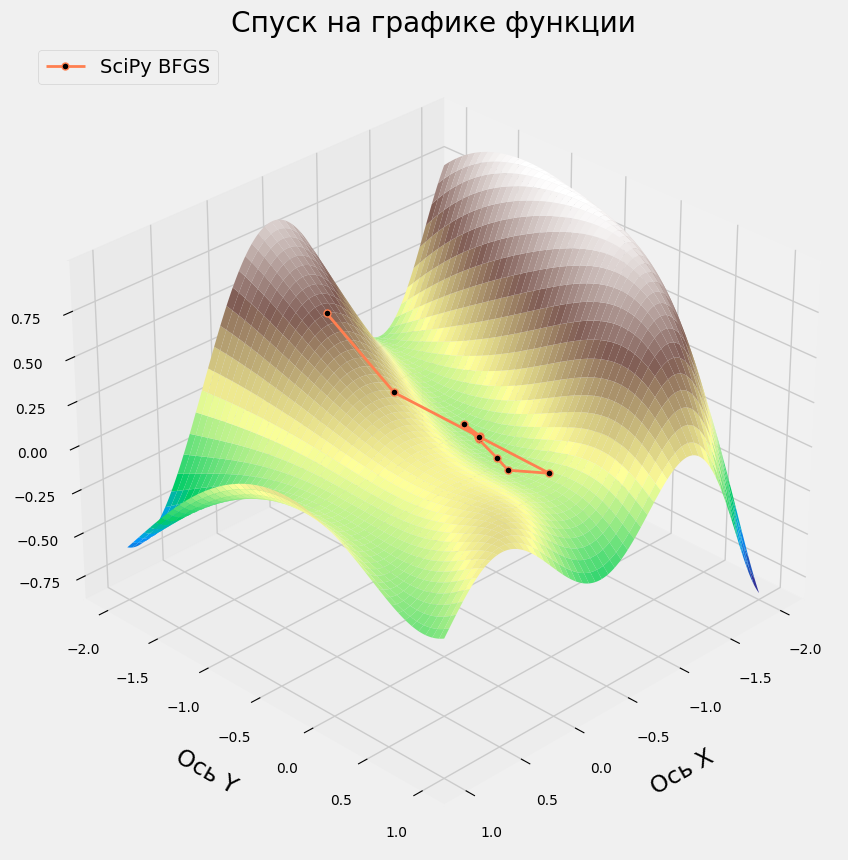
\includegraphics[scale = 0.35]{Image/T2A_F1_scipy_BFGS.png}
		\caption*{BFGS vs. SciPy's on first function}
	\end{figure}
	Как мы видим, собственная реализация, которая слева, первыми несколькими уверенными шагами почти доходит минимума, а затем начинает <<топтаться>> на месте в надежде на то, что он найдет самый-самый из минимумов.
	А с библиотечной реализацией чуть поинтереснее: он делает первые несколько шагов немного в сторону, но затем, сбавляя скорость (уменьшая размер шага), доходит и заканчивает свой алгоритм, из-за условия сходимости.
	Более наглядно можно разглядеть путь соперников в виде линий уровней:
	\begin{figure}[H]
		\centering
		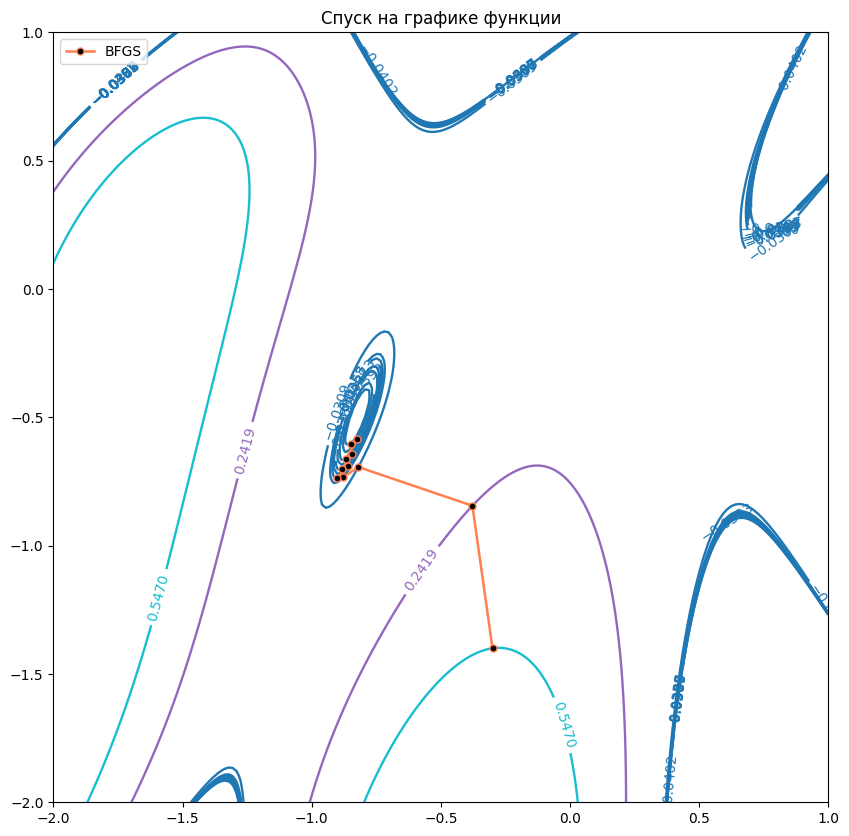
\includegraphics[scale = 0.35]{Image/T2A_F1_BFGS_LEVELS.png}
		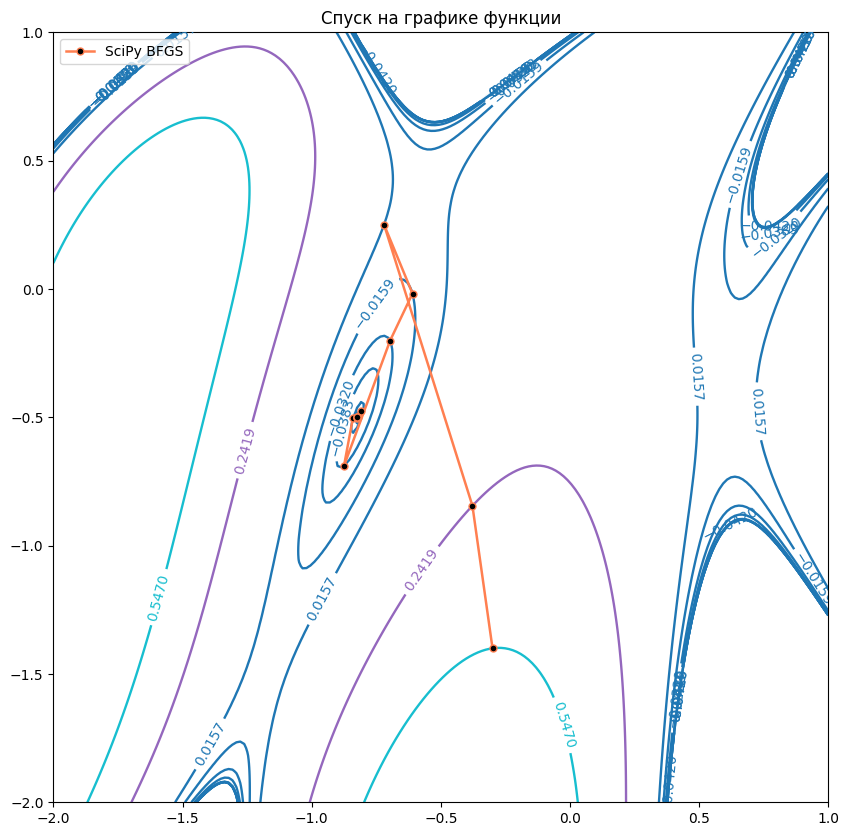
\includegraphics[scale = 0.35]{Image/T2A_F1_scipy_BFGS_LEVELS.png}
		\caption*{BFGS vs. SciPy's on first function (levels)}
	\end{figure}
	Наконец, посмотрим на полученные результаты работы в виде таблицы:
	\begin{table}[H]
		\centering
		\begin{tabular}{l|l|l|l}
			Испытуемый & Количество шагов & $\langle x, y \rangle$ & $z$ \\ \hline
			Собственная реализация & $11$ & $\langle -0.848456, -0.605206 \rangle$ & $-0.040723$ \\
			SciPy & $11$ & $\langle -0.822922, -0.499418 \rangle$ & $-0.041983$
		\end{tabular}
	\end{table}
	Теперь рассмотрим немного другую функцию, а именно~-- Химмельблау, у которого, как мы знаем, есть четыре эквивалентных минимума и определена она так:
	\[
		f(x, y) = \left(x^2 + y - 11\right)^2 + (x + y^2 - 7)^2
	\]
	Поставим здесь немного другие параметры на запуск алгоритмов:
	\begin{align*}
		\langle x_0, y_0 \rangle &= \langle 3.0, 0.5 \rangle~\text{(начальное приближение)} \\
		\mathtt{max\_iter} &= 13~\text{(максимальное количество шагов)}
	\end{align*}
	Запустим наших зверей на бедную функцию и посмотрим на вывод путей в трехмерном виде:
	\begin{figure}[H]
		\centering
		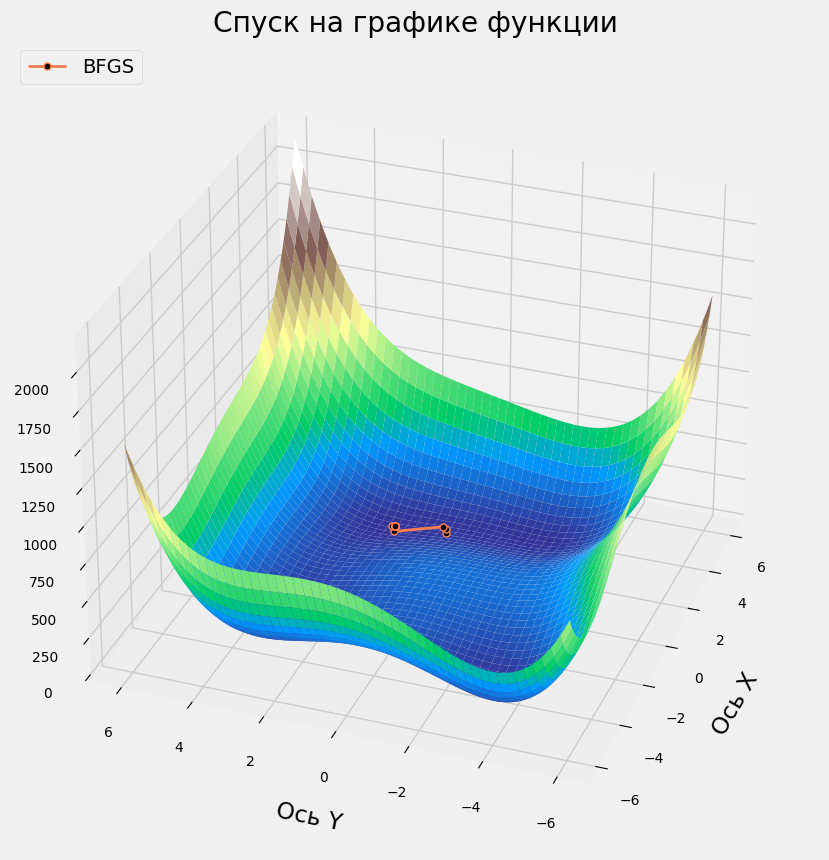
\includegraphics[scale = 0.35]{Image/T2A_F2_BFGS.png}
		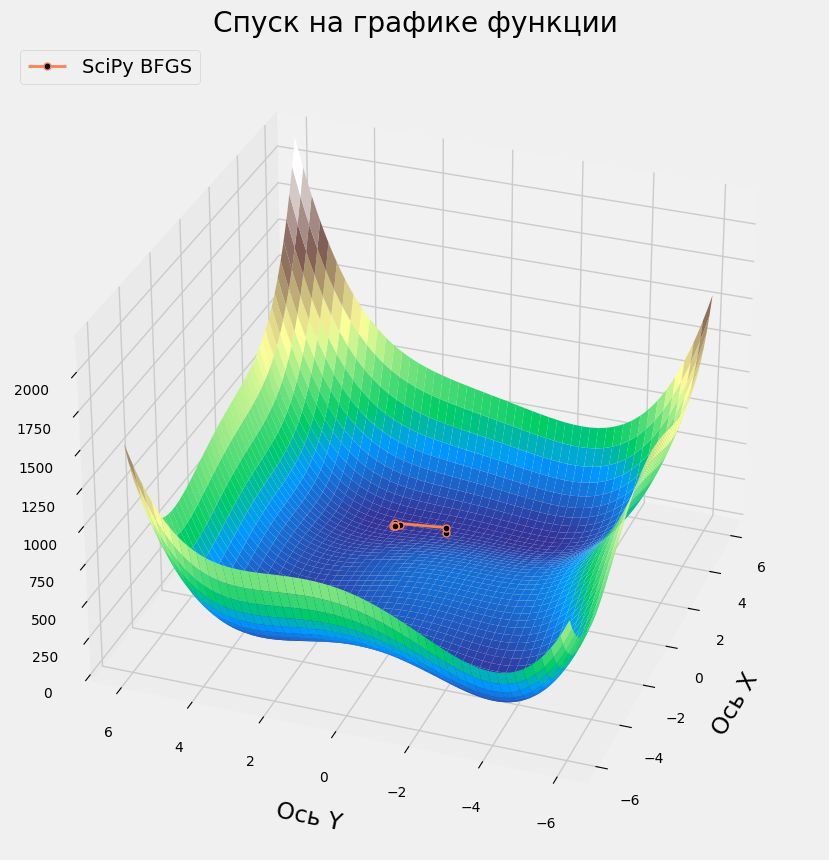
\includegraphics[scale = 0.35]{Image/T2A_F2_scipy_BFGS.png}
		\caption*{BFGS vs. SciPy's on second function}
	\end{figure}
	А вот здесь своя реализация, которая опять же слева, начинает проигрывать библиотеке.
	Заметим, что с начальной позиции алгоритм начал неестественно себя вести и делать, внезапно, слишком малые шаги до тех пор, пока не понял, что он не прав.
	Это связано с тем, что исходная точка лежит примерно в окрестности локального минимума относительно одной из четырех настоящих.
	При этом заметим, что написанный вариант вручную упирается в количество данных ему шагов.
	Библиотечная же реализация не ошибается и сразу делает уверенный шаг к предполагаемой точке, а в следующие еще несколько итераций приближает минимум к самому-самому.
	Более наглядно можно разглядеть путь соперников в виде линий уровней:
	\begin{figure}[H]
		\centering
		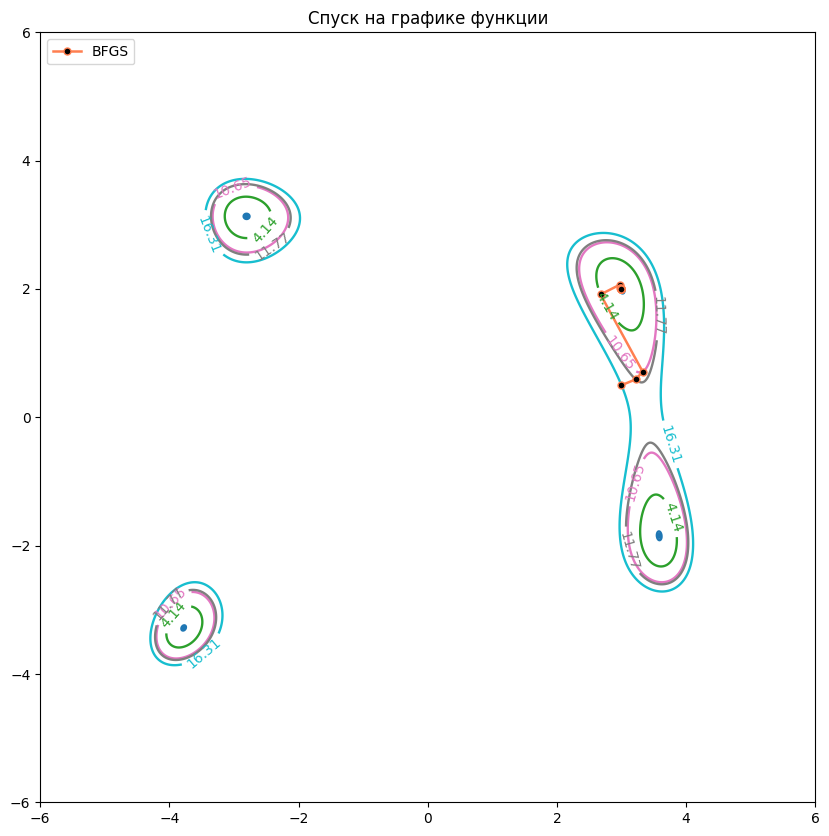
\includegraphics[scale = 0.35]{Image/T2A_F2_BFGS_LEVELS.png}
		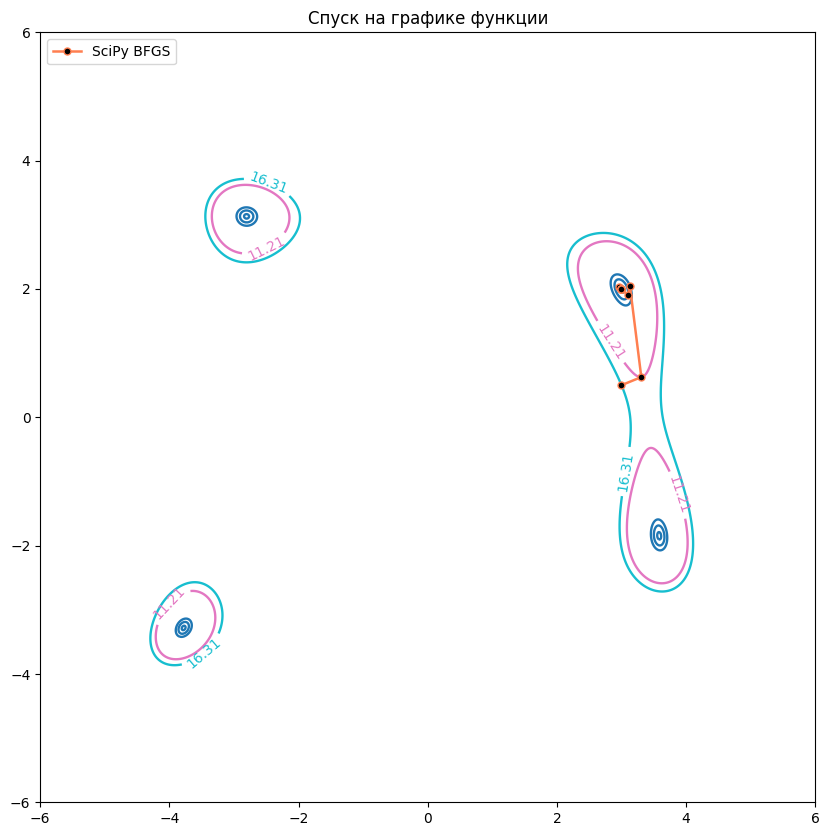
\includegraphics[scale = 0.35]{Image/T2A_F2_scipy_BFGS_LEVELS.png}
		\caption*{BFGS vs. SciPy's on second function (levels)}
	\end{figure}
	Наконец, посмотрим на полученные результаты работы в виде таблицы:
	\begin{table}[H]
		\centering
		\begin{tabular}{l|l|l|l}
			Испытуемый & Количество шагов & $\langle x, y \rangle$ & $z$ \\ \hline
			Собственная реализация & $14$ & $\langle 3.000000, 2.000000 \rangle$ & $0.000000$ \\
			SciPy & $10$ & $\langle 3.000000, 2.000000 \rangle$ & $0.000000$
		\end{tabular}
	\end{table}
	\paragraph{L-BFGS}
	Да-да, мы, конечно, обманули друг друга, сказав, что будет рассмотрен только BFGS, но тут мы просто обозначим и вспомним, что столь не очевидная модификация существует и пользуется популярностью, чем его предшественник.
	Функции и параметры мы возьмем теми же, поэтому, не будем на этом останавливаться и сразу выдадим результаты.
	Пути сходимости по первой функции:
	\begin{figure}[H]
		\centering
		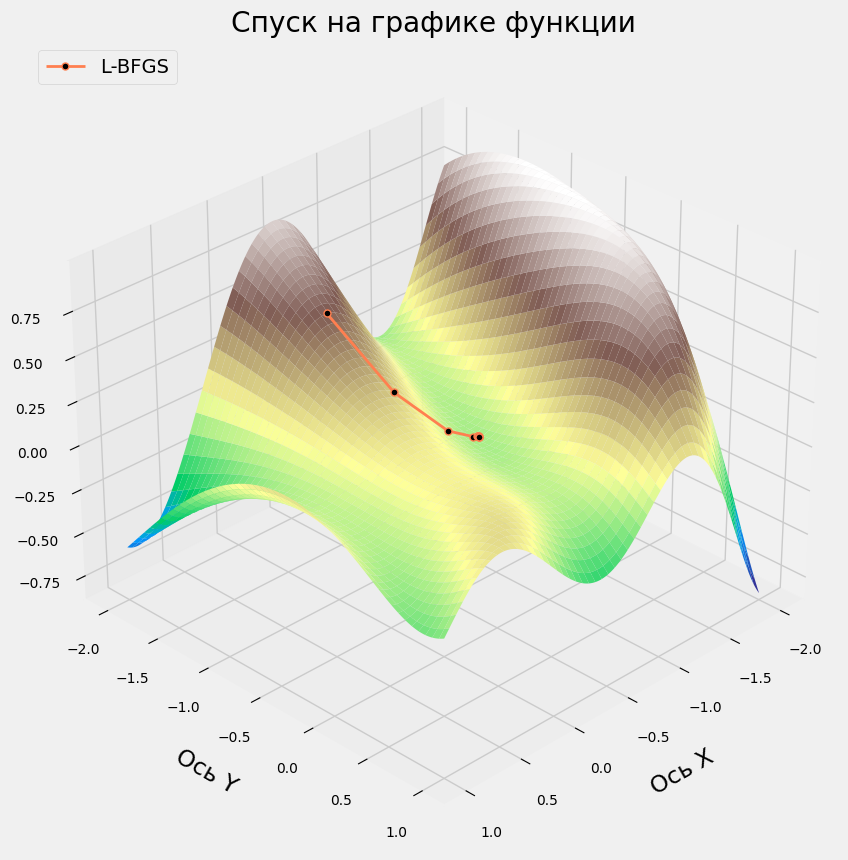
\includegraphics[scale = 0.35]{Image/T2A_F1_LBFGS.png}
		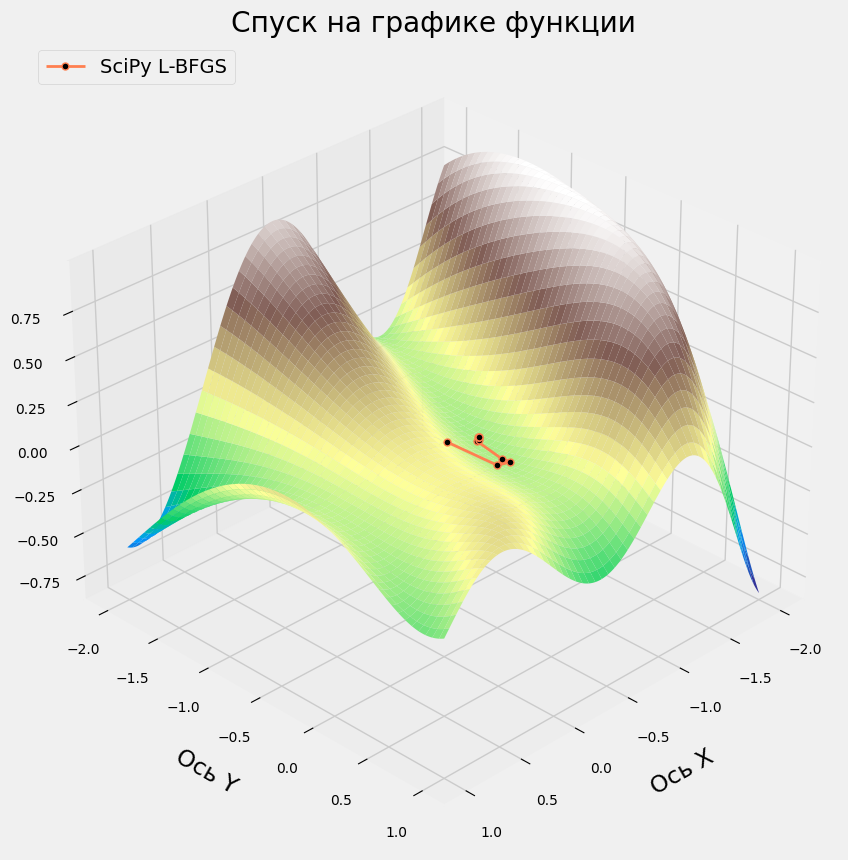
\includegraphics[scale = 0.35]{Image/T2A_F1_scipy_LBFGS.png}
		\caption*{L-BFGS vs. SciPy's on first function}
	\end{figure}
	Линии уровней путей сходимости по первой функции:
	\begin{figure}[H]
		\centering
		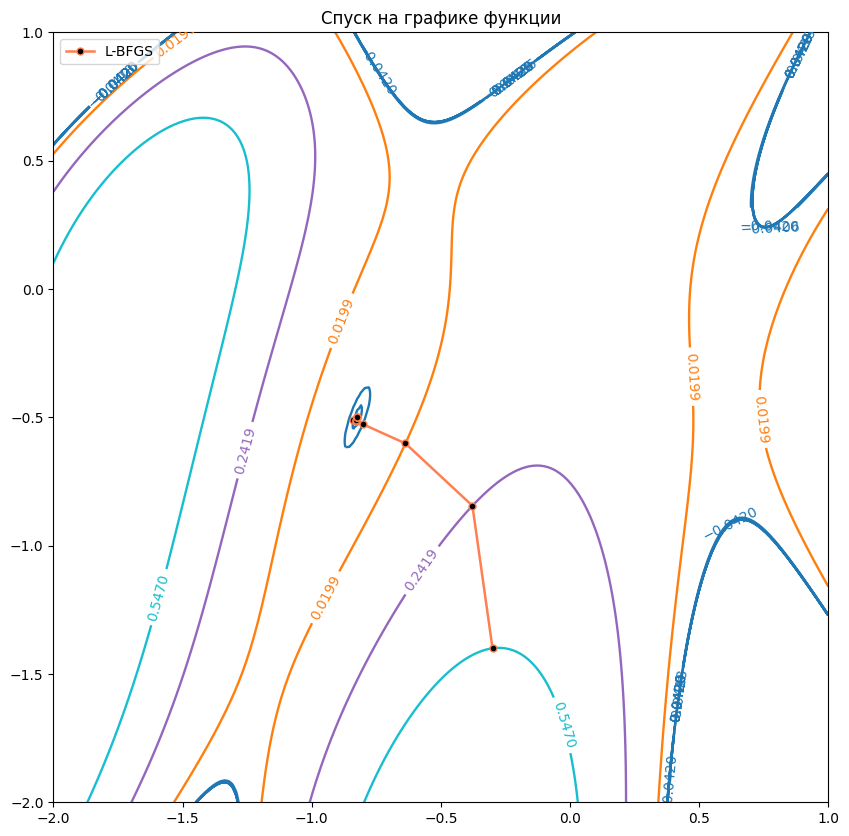
\includegraphics[scale = 0.35]{Image/T2A_F1_LBFGS_LEVELS.png}
		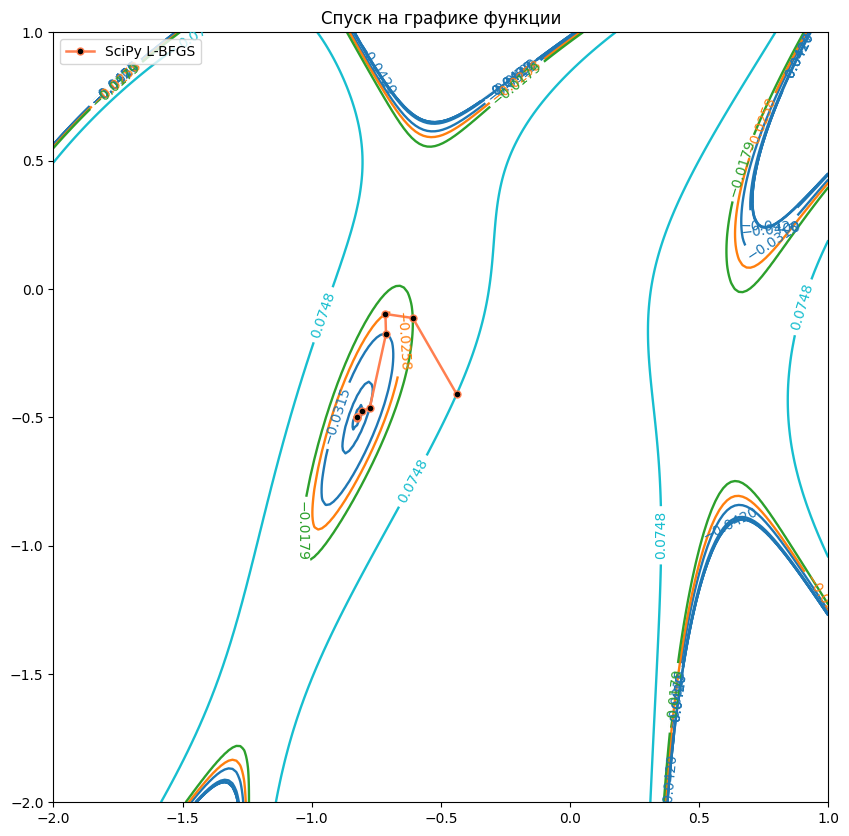
\includegraphics[scale = 0.35]{Image/T2A_F1_scipy_LBFGS_LEVELS.png}
		\caption*{L-BFGS vs. SciPy's on first function (levels)}
	\end{figure}
	Данные, полученные после схождения:
	\begin{table}[H]
		\centering
		\begin{tabular}{l|l|l|l}
			Испытуемый & Количество шагов & $\langle x, y \rangle$ & $z$ \\ \hline
			Собственная реализация & $10$ & $\langle -0.822934, -0.499453 \rangle$ & $-0.041983$ \\
			SciPy & $8$ & $\langle -0.822922, -0.499418 \rangle$ & $-0.041983$
		\end{tabular}
	\end{table}
	Теперь перейдем к второй функции.
	Пути сходимости алгоритмов:
	\begin{figure}[H]
		\centering
		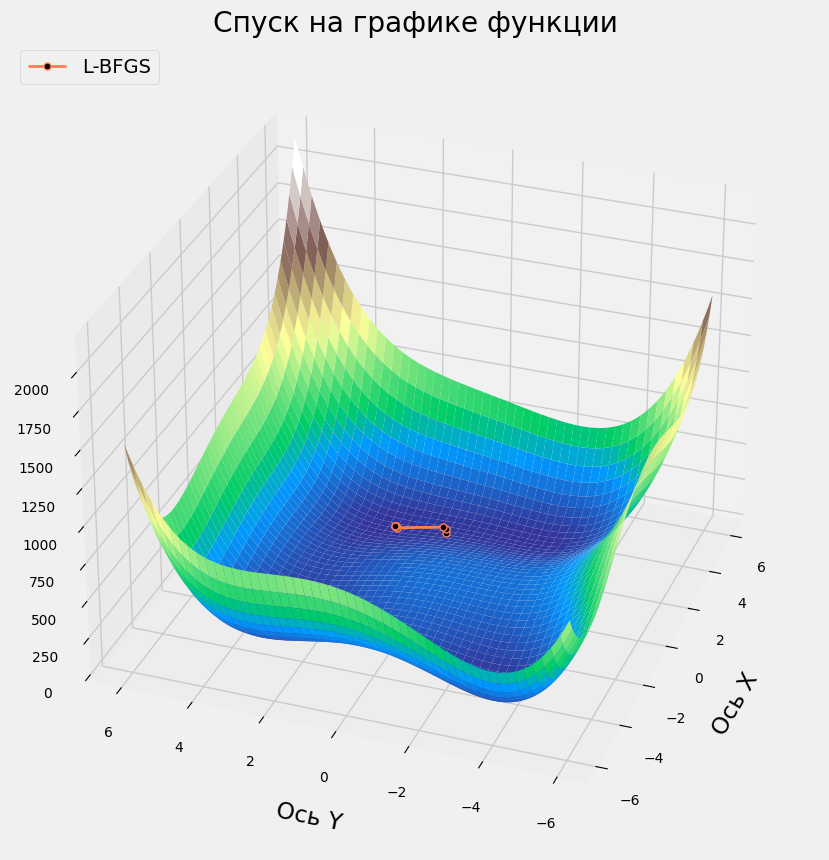
\includegraphics[scale = 0.35]{Image/T2A_F2_LBFGS.png}
		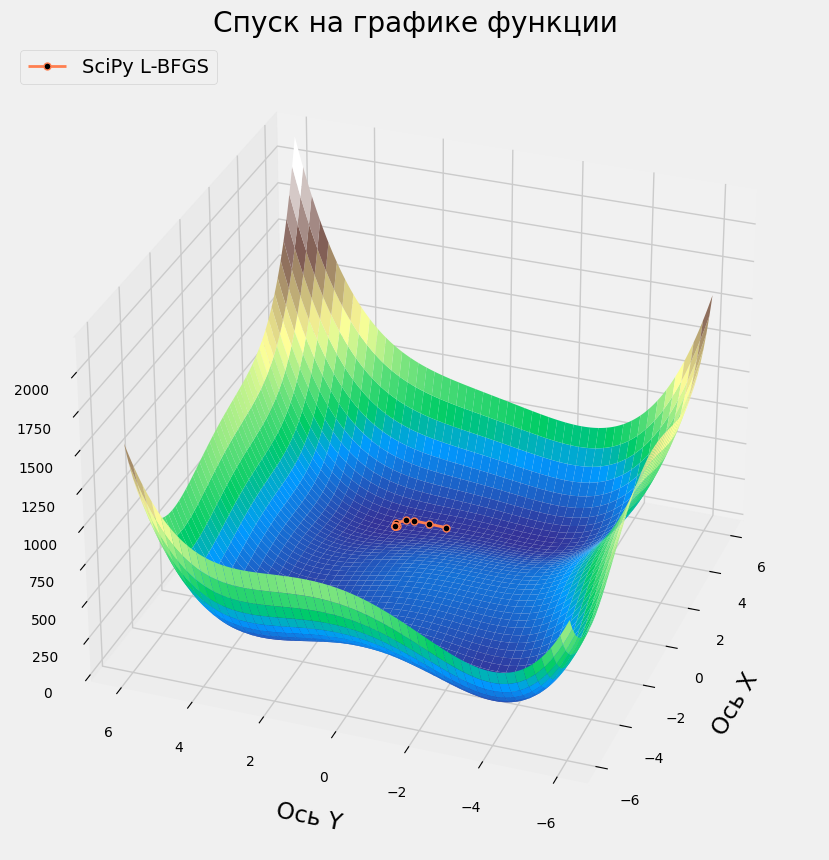
\includegraphics[scale = 0.35]{Image/T2A_F2_scipy_LBFGS.png}
		\caption*{L-BFGS vs. SciPy's on second function}
	\end{figure}
	Линии уровней путей сходимости:
	\begin{figure}[H]
		\centering
		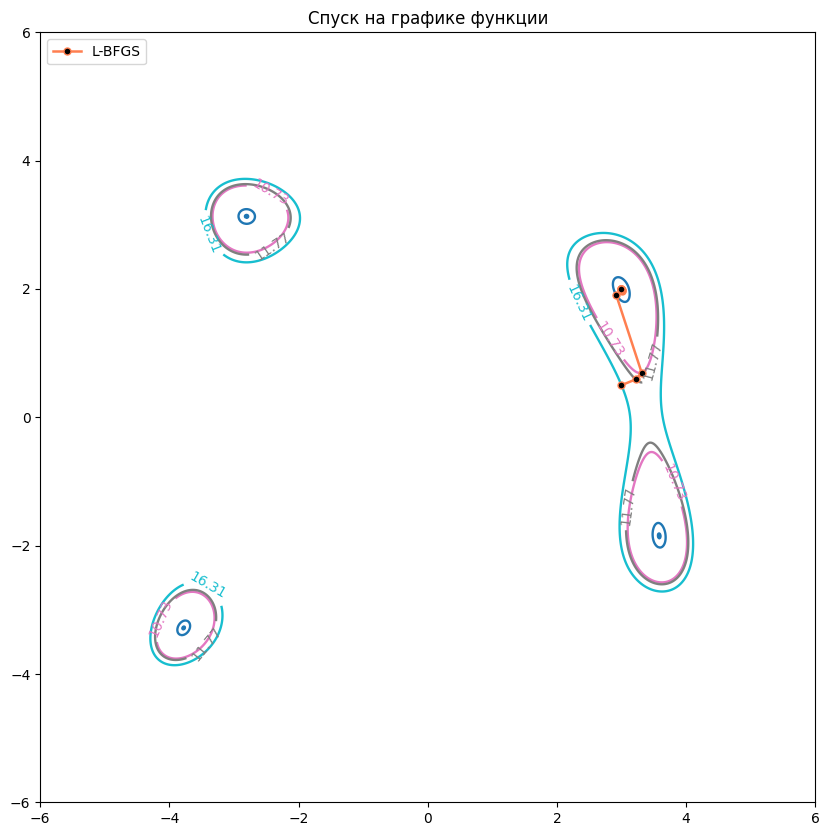
\includegraphics[scale = 0.35]{Image/T2A_F2_LBFGS_LEVELS.png}
		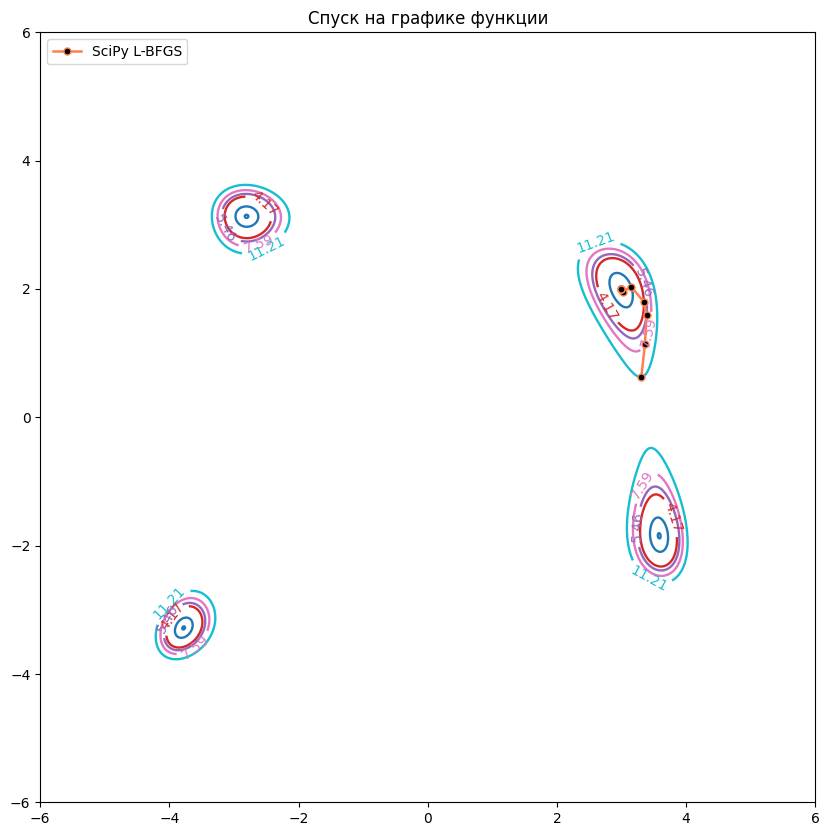
\includegraphics[scale = 0.35]{Image/T2A_F2_scipy_LBFGS_LEVELS.png}
		\caption*{L-BFGS vs. SciPy's on first function (levels)}
	\end{figure}
	Наконец, полученные после схождения данные:
	\begin{table}[H]
		\centering
		\begin{tabular}{l|l|l|l}
			Испытуемый & Количество шагов & $\langle x, y \rangle$ & $z$ \\ \hline
			Собственная реализация & $11$ & $\langle 3.000000, 2.000000 \rangle$ & $0.000000$ \\
			SciPy & $9$ & $\langle 3.000000, 2.000000 \rangle$ & $0.000000$
		\end{tabular}
	\end{table}
	\subsubsection*{vs. \mintinline{python}|scipy.optimize.least_squares|}
	\subsection*{Градиентный спуск PyTorch}
	Итак, поймем, что мы хотим от любого спуска к минимуму: чтобы градиент, который является неотъемлемой частью почти любого известного нам алгоритма минимизации значения, был более менее правдоподобен.
	Но здесь мы встречаемся лицом к лицу с проблемой, связанной с возможностями нашей системы и математики: мы не можем бесконечно долго манипулировать и что-либо другого делать с не целочисленным типами данных, они буду всё хуже и хуже деградировать от одной математической операции к другой.
	Поэтому, мы ставим задачу получить как можно лучший градиент и значение в этой точке более точно.

	Для примера мы рассмотрим функцию Розенброка и три метода получения градиента: из библиотеки \texttt{torch}, из \texttt{numdifftool}, и методом <<по определению>> в буквальном смысле.
	В качестве функции минимизации мы возьмем модификацию стохастического градиентного спуска Adam (из коллекции собственных реализаций), в качестве начальной точки $\langle p_{x_0}, p_{y_0} \rangle \gets \langle -1.0, 0.1 \rangle$, для всех разных методов получения градиента мы положим в качестве начального шага $\mathtt{initial\_w} = 0.5$ и, наконец, сгенерируем набор данных для исследования градиентов.
	\begin{figure}[H]
		\centering
		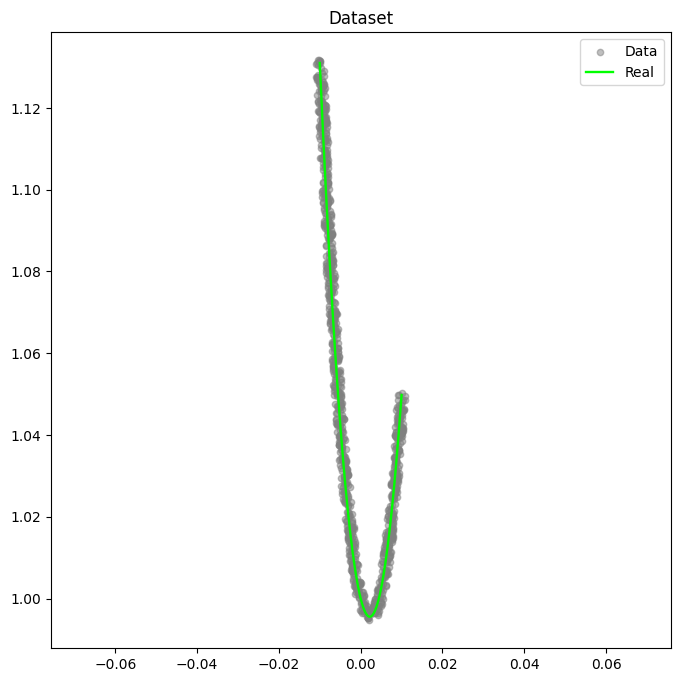
\includegraphics[scale = 0.65]{Image/T2B_DATASET.png}
		\caption*{Generated dataset for Rosen}
	\end{figure}
	Запустим наших зверей и посмотрим вот на какие результаты:
	\begin{table}[H]
		\centering
		\begin{tabular}{l|l}
			Выбранный метод градиента & Количество шагов до схождения \\ \hline
			<<По определению>>        & $51$ \\
			\texttt{torch}            & $51$ \\
			\texttt{numdifftool}      & $51$
		\end{tabular}
	\end{table}
	Замечаем интересную находку: все использованные методы сходятся за одинаковое число шагов, умоляя общности среднего подсчета, что нам явно гарантирует, что мы можем использовать любой из них и, при любом раскладе, выиграть.
	Теперь же мы посмотрим на разницу отношения текущей приближенной точки алгоритма и её градиента для всех трех методов.
	Зададим в качестве обозначений $\langle p_x, p_y\rangle$~- точка, $\langle t_x, t_y\rangle$~- градиент из \texttt{torch}, $\langle n_x, n_y\rangle$~- градиент из \texttt{numdifftool} и $\langle d_x, d_y\rangle$~- градиент по определению.
	Полученные результаты для \texttt{torch}, здесь и далее будут выведены первые и последние четыре измерения.:
	\begin{table}[H]
		\centering
		\begin{tabular}{c|c}
			$\langle p_x, p_y \rangle$ & $\langle t_x, t_y \rangle$ \\ \hline
			$\langle -1.0, ~ 0.1 \rangle$ & $\langle -0.00146706559993418353, ~ -0.00014721156217214419 \rangle$ \\
			$\langle -0.58826355, ~ 0.14131537 \rangle$ & $\langle -0.00131440381006264718, ~ -0.00019862055015740611 \rangle$ \\
			$\langle -0.14727034, ~ 0.19673504 \rangle$ & $\langle -0.00115017868324561500, ~ -0.00026529536789049484 \rangle$ \\
			$\langle 0.29978107, ~ 0.2682456 \rangle$ & $\langle -0.00098270545906175904, ~ -0.00034802171851757964 \rangle$ \\
			$\vdots$ & $\vdots$ \\
			$\langle 1.79226672, ~ 3.02522473 \rangle$ & $\langle -0.00008879931707961148, ~ 0.00002868576216914081 \rangle$ \\
			$\langle 1.81834509, ~ 3.03876149 \rangle$ & $\langle -0.00007504682716224205, ~ 0.00008702729437093851 \rangle$ \\
			$\langle 1.8468342, ~ 3.04139108 \rangle$ & $\langle -0.00006181034719901721, ~ 0.00012621921750756307 \rangle$ \\
			$\langle 1.87666167, ~ 3.03296134 \rangle$ & $\langle -0.00005016024349737770, ~ 0.00013933684458654905 \rangle$
		\end{tabular}
	\end{table}
	Полученные результаты для \texttt{numdifftool}:
	\begin{table}[H]
		\centering
		\begin{tabular}{c|c}
			$\langle p_x, p_y \rangle$ & $\langle n_x, n_y \rangle$ \\ \hline
			$\langle -1.0, ~ 0.1 \rangle$ & $\langle -0.00146706559993418201, ~ -0.00014721156217214299 \rangle$ \\
			$\langle -0.58826355, ~ 0.14131537 \rangle$ & $\langle -0.00131440381006265347, ~ -0.00019862055015741075 \rangle$ \\
			$\langle -0.14727034, ~ 0.19673504 \rangle$ & $\langle -0.00115017868324561912, ~ -0.00026529536789049452 \rangle$ \\
			$\langle 0.29978107, ~ 0.2682456 \rangle$ & $\langle -0.00098270545906175687, ~ -0.00034802171851757129 \rangle$ \\
			$\vdots$ & $\vdots$ \\
			$\langle 1.79226672, ~ 3.02522473 \rangle$ & $\langle -0.00008879931707961108, ~ 0.00002868576216914129 \rangle$ \\
			$\langle 1.81834509, ~ 3.03876149 \rangle$ & $\langle -0.00007504682716224151, ~ 0.00008702729437093872 \rangle$ \\
			$\langle 1.84683428, ~ 3.04139108 \rangle$ & $\langle -0.00006181034719901730, ~ 0.00012621921750756380 \rangle$ \\
			$\langle 1.87666167, ~ 3.03296134 \rangle$ & $\langle -0.00005016024349737770, ~ 0.00013933684458654840 \rangle$
		\end{tabular}
	\end{table}
	Полученные результаты для собственного градиента:
	\begin{table}[H]
		\centering
		\begin{tabular}{c|c}
			$\langle p_x, p_y \rangle$ & $\langle d_x, d_y \rangle$ \\ \hline
			$\langle -1.0, ~ 0.1 \rangle$ & $\langle -0.00146706560007897613, ~ -0.00014721156195093843 \rangle$ \\
			$\langle -0.58826355, ~ 0.14131537 \rangle$ & $\langle -0.00131440380931810430, ~ -0.00019862055056218964 \rangle$ \\
			$\langle -0.14727034, ~ 0.19673504 \rangle$ & $\langle -0.00115017868319855499, ~ -0.00026529536813896248 \rangle$ \\
			$\langle 0.29978107, ~ 0.2682456 \rangle$ & $\langle -0.00098270545867418235, ~ -0.00034802171864842246 \rangle$ \\
			$\vdots$ & $\vdots$ \\
			$\langle 1.79226672, ~ 3.02522473 \rangle$ & $\langle -0.00008879931708840553, ~ 0.00002868576212612835 \rangle$ \\
			$\langle 1.81834509, ~ 3.03876149 \rangle$ & $\langle -0.00007504682706977080, ~ 0.00008702729432008473 \rangle$ \\
			$\langle 1.84683428, ~ 3.04139108 \rangle$ & $\langle -0.00006181034720512124, ~ 0.00012621921753218010 \rangle$ \\
			$\langle 1.87666167, ~ 3.03296134 \rangle$ & $\langle -0.00005016024348539292, ~ 0.00013933684456614911 \rangle$
		\end{tabular}
	\end{table}
	\subsection*{Эксперименты с SciPy}
	\newpage
	\section*{Линейные и нелинейные ограничения}
\end{document}
